\chapter{基于改进的RetinaNet骨髓血细胞检测算法设计与实现}
\section{引言}

第三章中,我们对比了多个单阶段与双阶段检测网络在骨髓血细胞数据上的性能,综合考虑计算量,参数量与检测精度等因素,
我们选择将性能优异的RetinaNet作为基线模型。此外我们确定了先检测再识别的骨髓血细胞处理流程,即检测网络只需要
对血细胞进行前景检测与坐标回归。在RetianNet基线模型中,尽管模型的检测精度已经很高,但仍然存在着漏检、密集与重叠的血细胞区域
边界检测错误等问题,如图~\ref{fig:detect_problem}所示。

骨髓血细胞检测主要有如下三个难点:(1)相比外周血红细胞、白细胞、血小板三类血细胞检测,骨髓血细胞种类繁多、
形态丰富,尺寸大小不一。(2)在骨髓涂片制作过程中,由于染色剂与光照条件的变化,多个批次的数据存在着色彩差异。此外图像
背景复杂,存在较多成熟红细胞的干扰。(3)对于骨髓细胞增生活跃的切片,存在大量血细胞密集堆叠,边缘黏连,易导致漏检、错检等问题。
因此精准检测到骨髓血细胞是一项十分具有挑战性的课题。

针对上述难点与基线模型中存在的问题,本章提出了一种改进RetinaNet网络。该方法中,我们提出了一种基于全局注意力的自底向上的路径聚合网络结构,
缩短了底层与顶层特征之间的信息传递路径,提升网络对位置特征的提取能力。此外探究了不同标签分配策略对检测性能的影响,
提出基于最优输运的标签策略用于密集区域的血细胞的标签分配,避免了模糊分配样本的出现,提高网络对血细胞的召回能力。
% 最后我们比较了空洞卷积、深度可分离卷积、可变形卷积等卷积网络,以期实现速度与检测精度的更优平衡。
在骨髓血细胞数据集上的实验结果表明,本文提出的改进方法在检测准确率上有较大的提升,达到了较为先进的性能。

\begin{figure}[htbp]                     
  \centering                      
  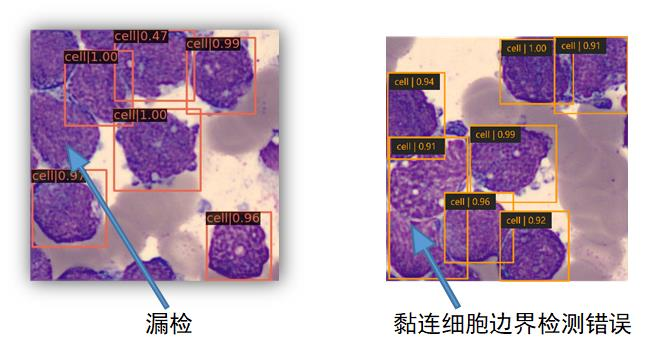
\includegraphics[width=0.7\linewidth]{detect_problem.jpg}                      
  \caption{RetinaNet基线模型检测错误示例}                      
  \label{fig:detect_problem}       
\end{figure}  

\section{改进的RetinaNet骨髓血细胞检测网络}
本章提出的改进RetinaNet网络结构如图~\ref{fig:improved_retinanet}所示,整体网络结构基于第三章的RetinaNet基线模型进行改进。骨干网络为
ResNet50用于图像特征提取,特征金字塔结构用于多尺度特征提取。锚框的尺寸、数量与分类回归网络结果与基线模型相同。
为了提高网络检测的精度,我们在特征金字塔后引入了自底向上的路径聚合模块,该模块基于全局注意力将更浅层的特征与FPN深层的进行融合,
提升网络定位特征的表达能力,此外我们引入了IOU预测分支,将检测框的定位质量也纳入到候选框的筛选中。
在训练过程中,我们使用基于最优输运的策略进行标签分配。
下面各个小节将详细介绍我们的改进点。
\begin{figure}[htbp]                     
  \centering                      
  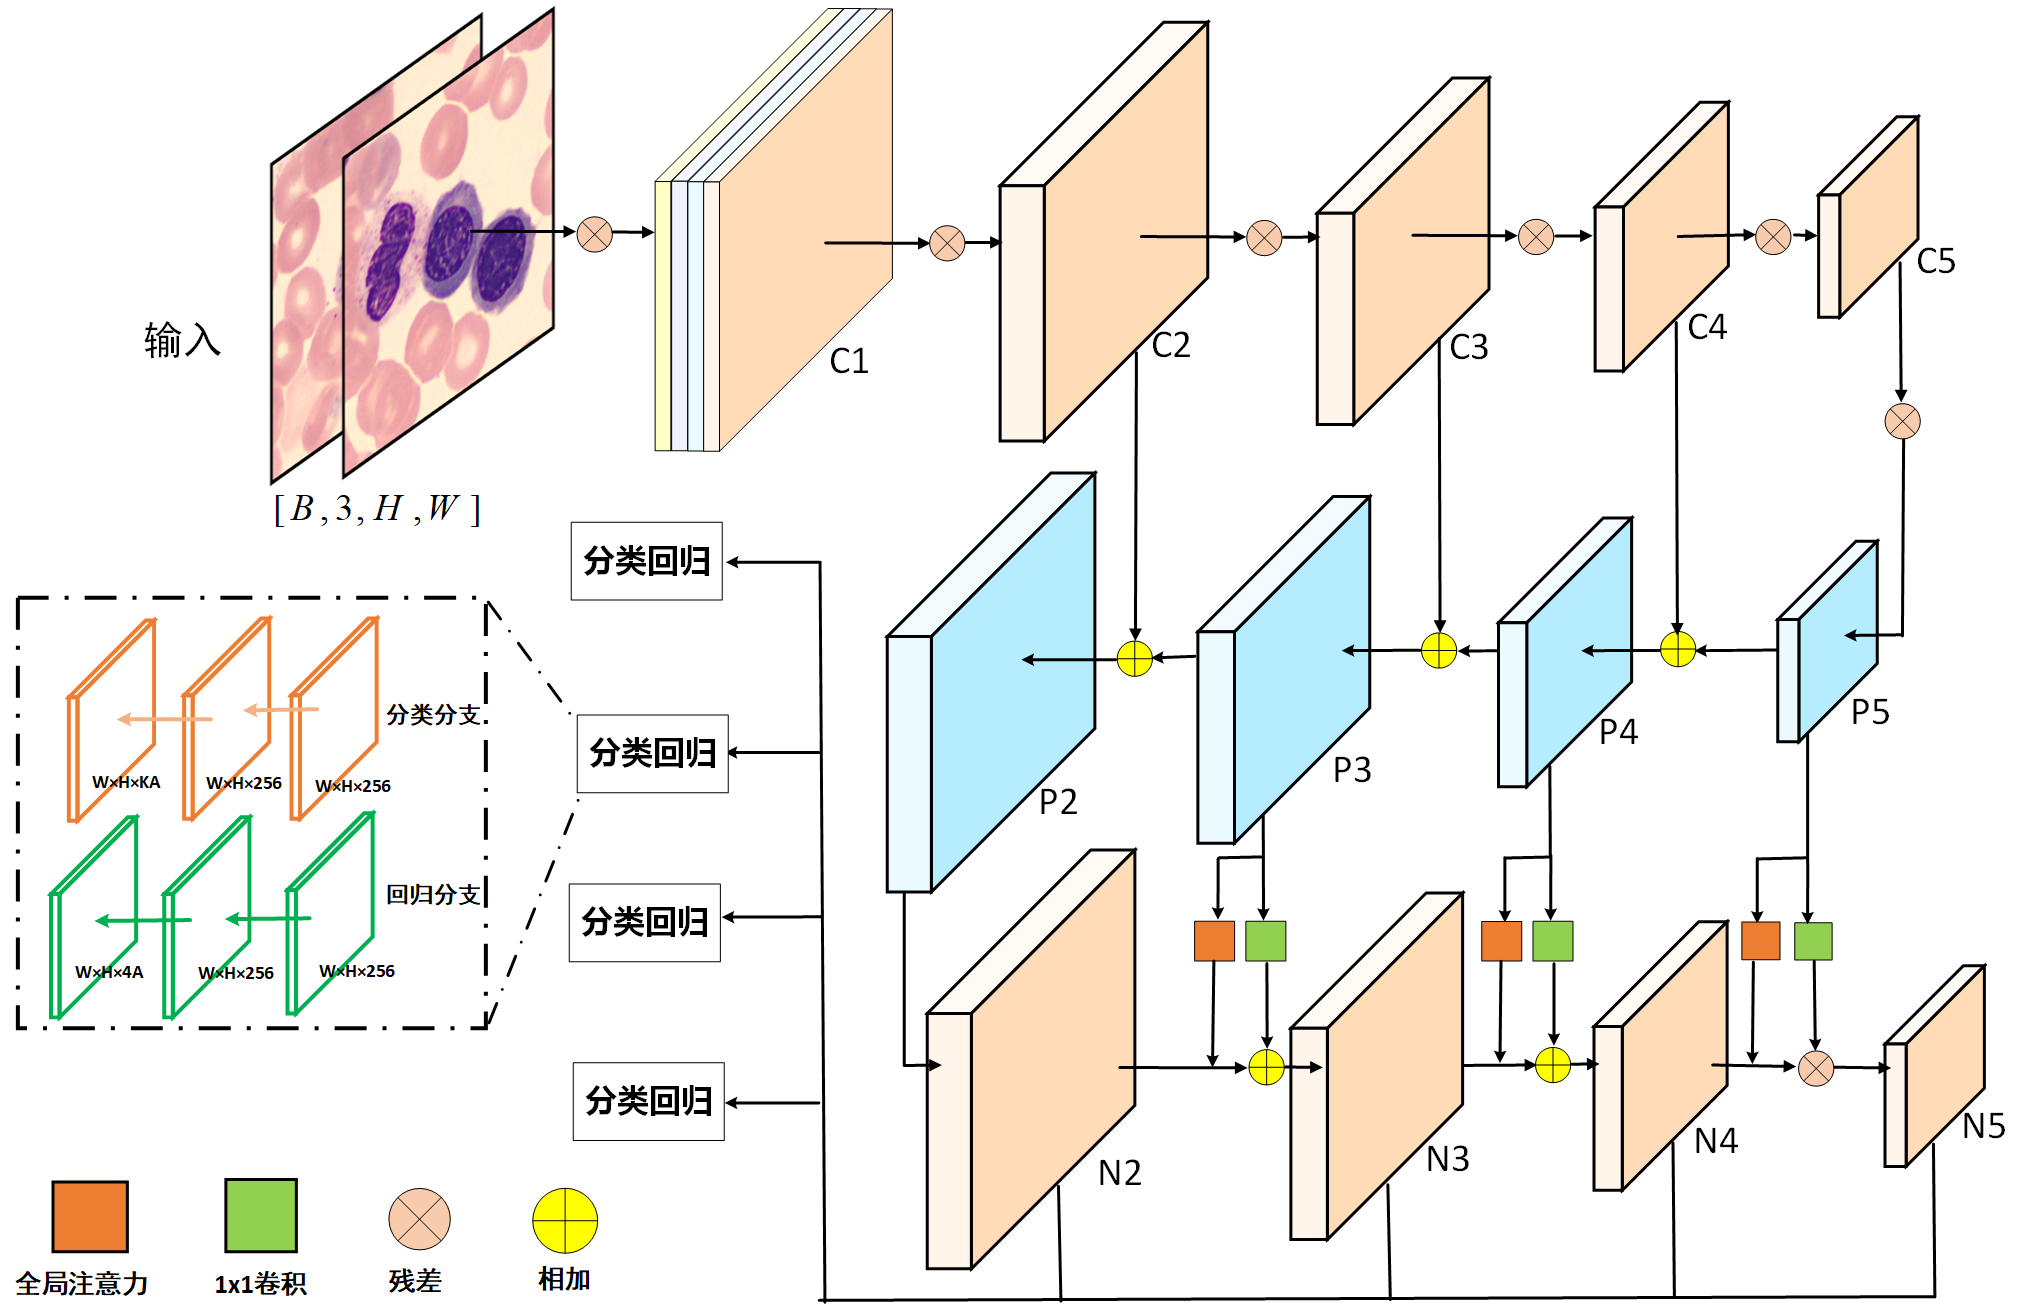
\includegraphics[width=0.95\linewidth]{improved_retinanet.png}                      
  \caption{改进的RetinaNet网络结构示意图}                      
  \label{fig:improved_retinanet}       
\end{figure}  

\subsection{基于全局注意的路径聚合网络}
ResNet50骨干网络提取了不同层级与尺度的特征图,高层次的特征图表达目标的抽象语义信息,低层次的特征图表达局部的纹理与模式信息,因此引入了
特征金字塔网络,增加自上而下的路径来传播语义强的特征,从而增强所有层次特征的分类能力。在骨髓血细胞检测任务中,我们更加关注网络对于血细胞
定位的准确性,这些定位信息主要存在浅层特征图的边缘、纹理信息中。我们构建了自底向上的路径聚合网络,将浅层的特征与特征金字塔深层的特征图
进行融合,通过特征直连缩短了底层到顶层特征之间的信息传递路径。原始结构中底层到顶层需要需要约50层网络,如图~\ref{fig:panet}红线所示。自下而上的路径聚合网络引入了
特征直连,从底层到顶层的路径只有不到10层,如图~\ref{fig:panet}绿线所示,该路径使得浅层的纹理等高分辨定位信息可以更有效的传递到顶层,
提升网络定位特征的表达能力。
\begin{figure}[htbp]                     
  \centering                      
  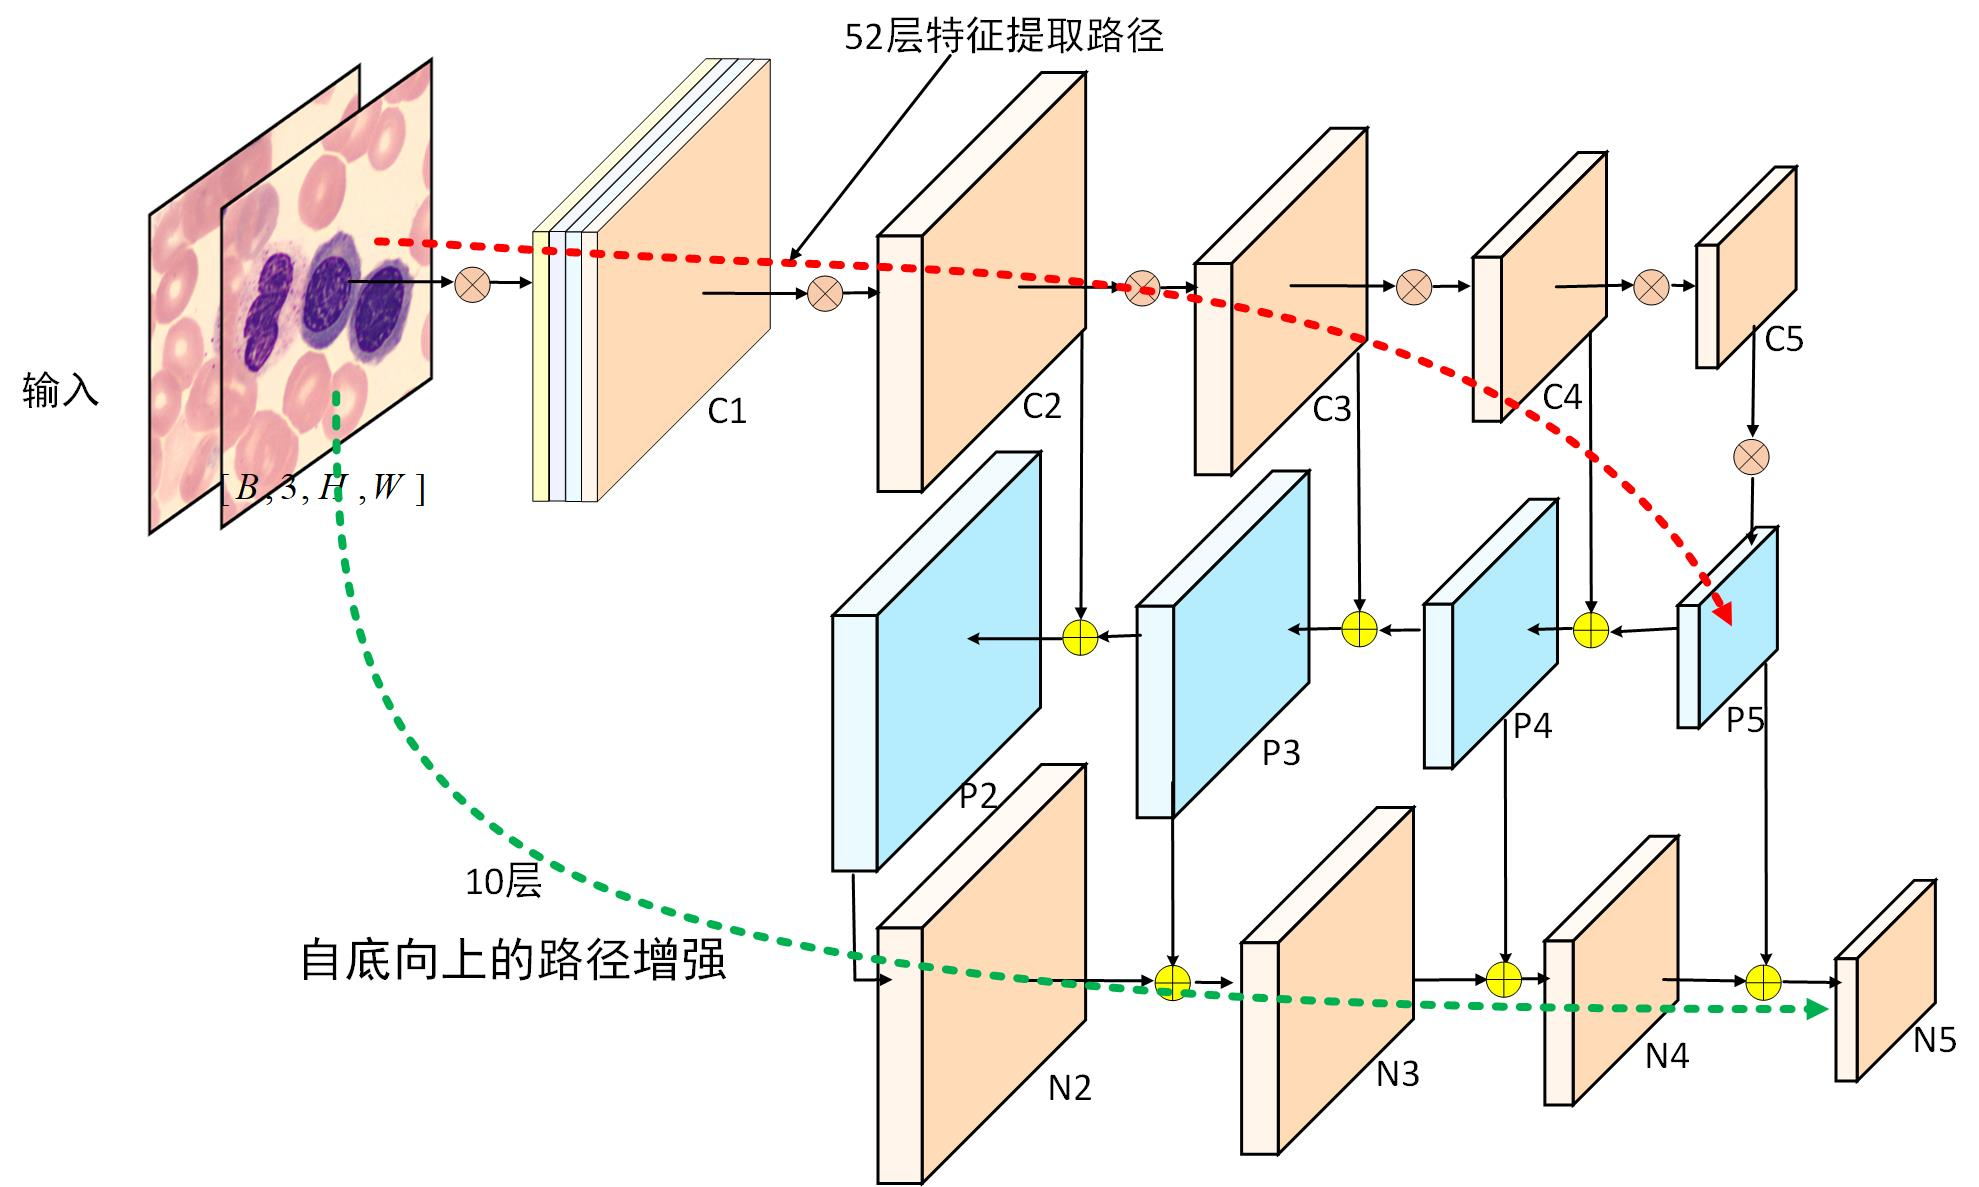
\includegraphics[width=0.75\linewidth]{panet.jpg}                      
  \caption{路径聚合网络结构示意图}                      
  \label{fig:panet}       
\end{figure}  

图中${C_2, C_3, C_4, C_5}$为ResNet50骨干网络不同阶段生成的特征图,${P_2, P_3, P_4, P_5}$为特征金字塔生成的不同级别的特征图。
自底向上的路径聚合网络从最底层的P2特征图开始,通过步长为2的卷积进行下采样并与高层的特征融合后生成新的特征图${N_2, N_3, N_4, N_5}$。
路径构建模块中使用了全局通道注意力机制\cite{li2018pyramid},使用全局上下文信息的高层次特征指导浅层特征的筛选,该结构如图~\ref{fig:gau}所示。

\begin{figure}[htbp]                     
  \centering                      
  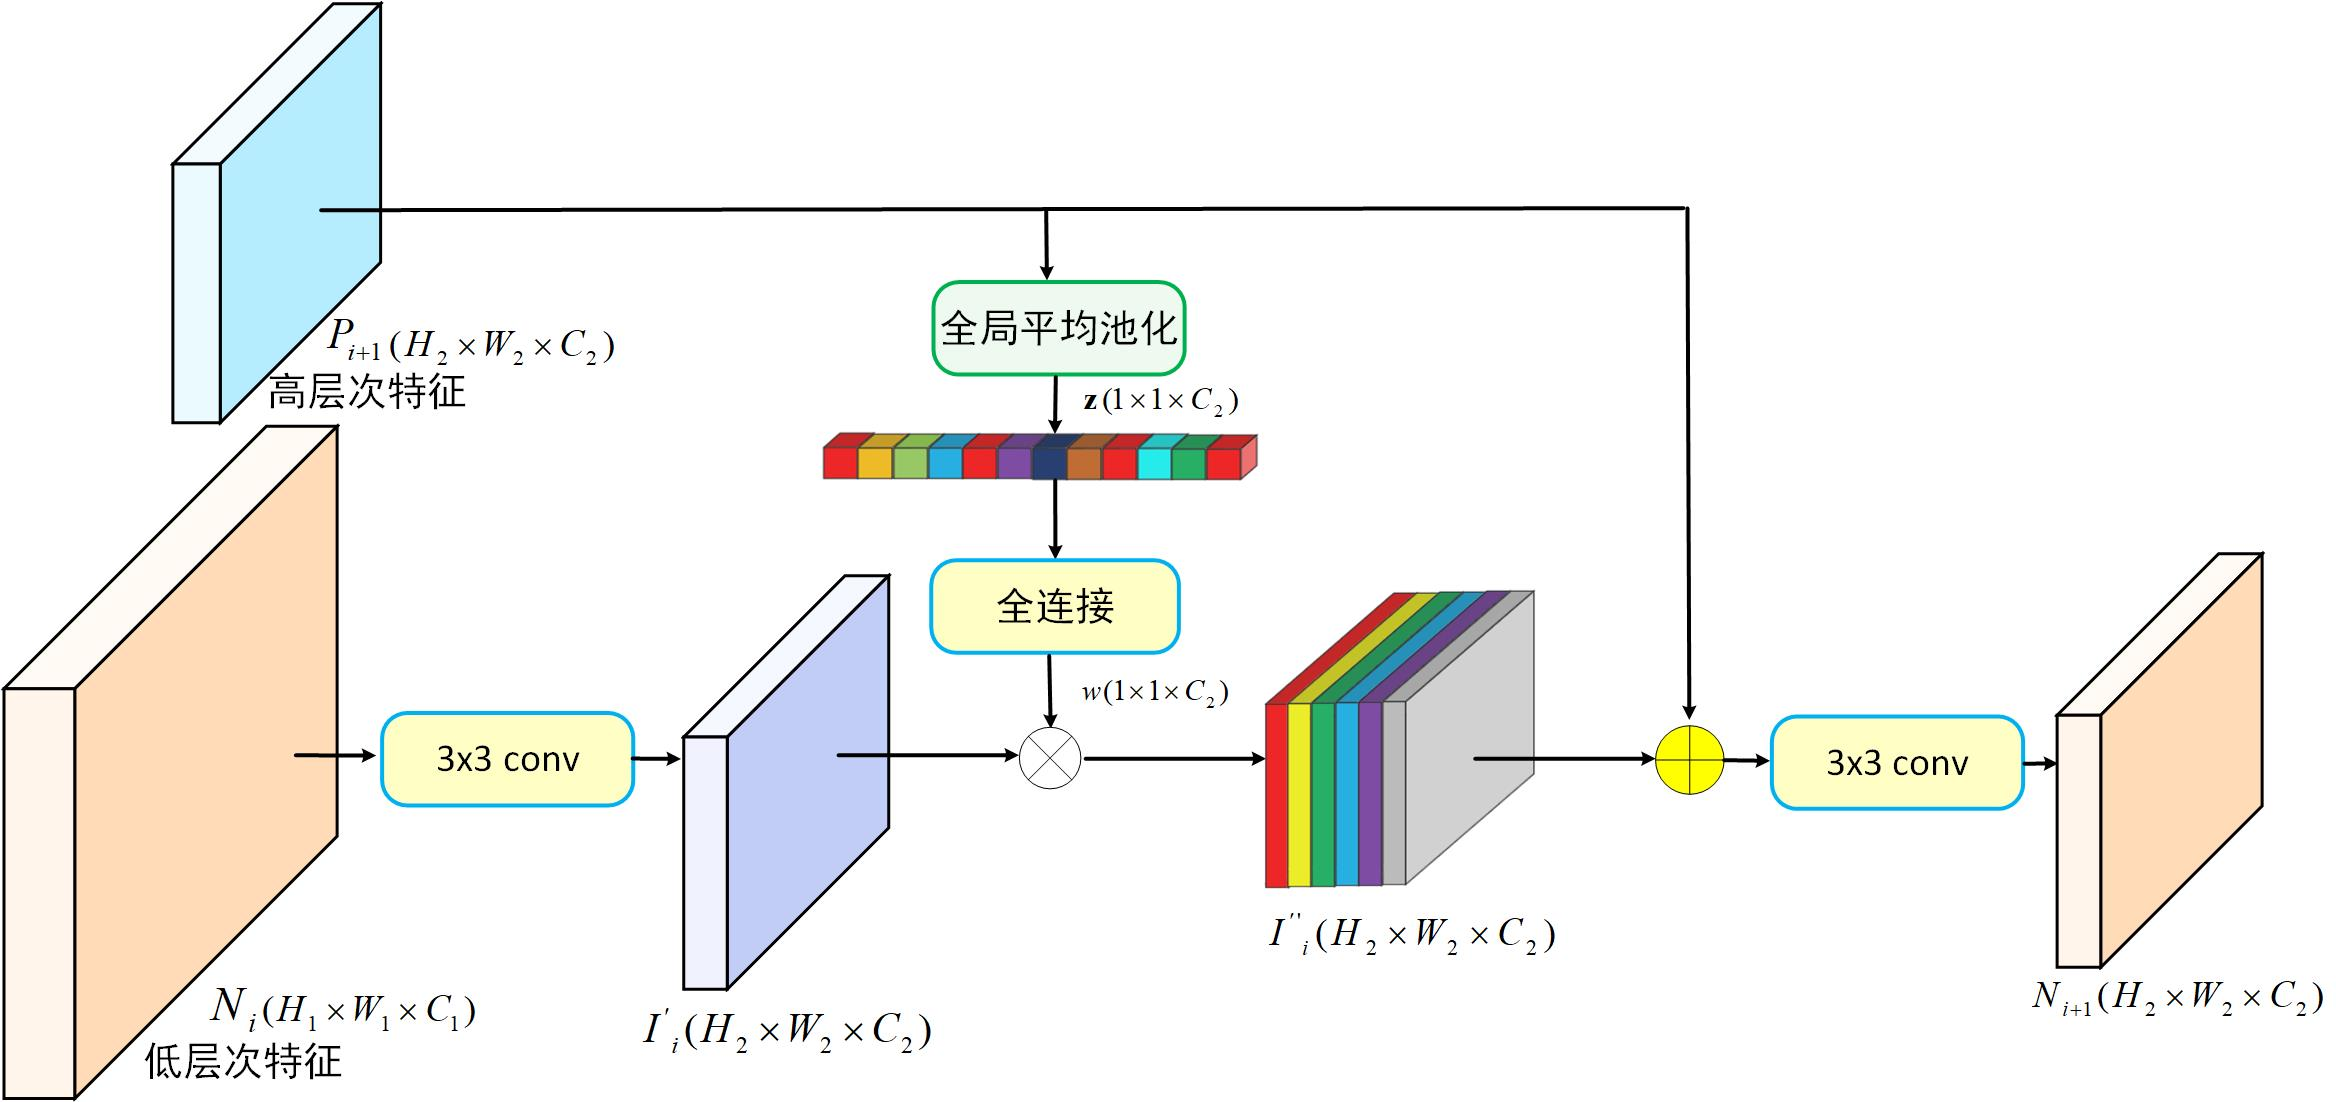
\includegraphics[width=0.95\linewidth]{gau.jpg}                      
  \caption{全局注意力模块}                      
  \label{fig:gau}       
\end{figure}  

全局注意力模块的输入分别是路径聚合网络的低层级特征图$N_i(H_1 \times W_1 \times C_1)$与特征金字塔的高层级特征图
$P_{i + 1}(H_2 \times W_2 \times C_2)$,输出新的特征图$N_{i + 1}$。首先对特征图$N_i$经过$3\times 3$、步长为2
的卷积层降低特征图的尺寸得到$I^{\prime}_i({H_2} \times {W_2} \times {C_2})$。对高层级的特征图$P_{i + 1}$进行全局
平均池化,每个通道压缩为一个值得到C维向量$z(1 \times 1 \times {C_2})$,如式~\ref{eq:squeeze}所示:
\begin{equation}   
  \mathbf{z} = {{\bf{F}}_{sq}}\left( {{{\bf{P}}_{i + 1}}} \right) = \frac{1}{{H \times W}}\sum\limits_{i = 1}^H {\sum\limits_{j = 1}^W {{{\bf{P}}_{i + 1}}} } (i,j)
  \label{eq:squeeze} 
\end{equation}

然后使用两层全连接结构来全局建模通道之间的依赖关系,第一层全连接的输出使用ReLU激活函数,第二层使用Sigmoid激活函数,得到权重
$\mathbf{w}(1 \times 1 \times {C_2})$,如式~\ref{eq:excitation}所示。
\begin{equation}   
  {\bf{w}} = {{\bf{F}}_{ex}}({\bf{z}},{\bf{W}}) = \sigma (g({\bf{z}},{\bf{W}})) = \sigma \left( {{{\bf{W}}_2}\delta \left( {{{\bf{W}}_1}{\bf{z}}} \right)} \right)
  \label{eq:excitation} 
\end{equation}

将权重向量$\mathbf{w}$与和特征$I^{\prime}_i({H_2} \times {W_2} \times {C_2})$按通道点乘得到加权后的特征$I^{\prime \prime}_i({H_2} \times {W_2} \times {C_2})$,
如式~\ref{eq:scale}所示。
\begin{equation}   
  {\bf{I}}_i^{\prime \prime } = {{\bf{F}}_{{\rm{scale }}}}\left( {{\bf{I}}_i^\prime ,{\bf{w}}} \right) = {w_c}I^\prime_{ic}
  \label{eq:scale} 
\end{equation}

将$\bf{I}_i^{\prime \prime}$与$P_{i + 1}$逐元素相加后再经过一个$3\times3$卷积层后得到路径聚合网络的下一层特征图$N_{i + 1}$。
不断迭代上述过程,直到生成$N_5$特征图为止。最终在融合后新的特征图$N_2, N_3, N_4, N_5$上进行区域提取与坐标回归。
anchor生成与分类回归结构与RetianNet相同,在第三章已进行详细解释。

\subsection{IOU预测分支}
RetinaNet在预测阶段会生成密集的检测框,这些检测框会按照置信度高低进行非极大值抑制(NMS),去除重复的检测框。上述NMS方式默认了一种假设,就是
置信度高的锚框定位也会更加精确。
\begin{figure}[htbp]
	\centering
  \begin{subfigure}{0.35\linewidth}
    \centering
    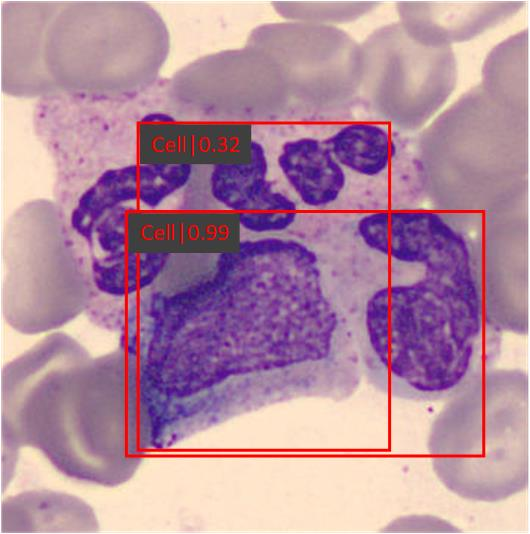
\includegraphics[width=0.95\linewidth, height=0.95\linewidth]{cell1.jpg}
    \caption{}
  \end{subfigure}
	\centering
	\begin{subfigure}{0.35\linewidth}
		\centering
		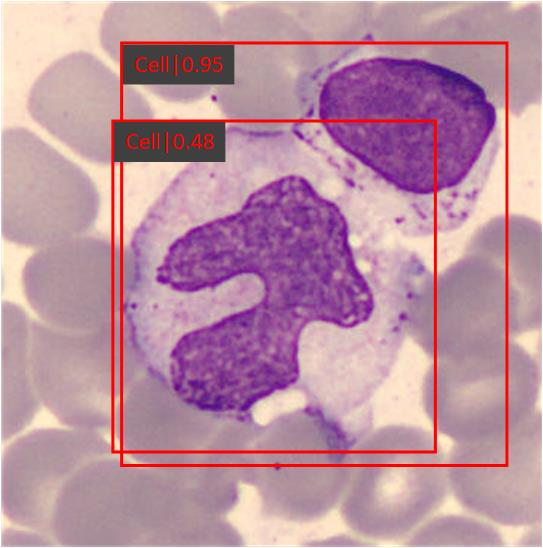
\includegraphics[width=0.95\linewidth, height=0.95\linewidth]{cell2.jpg}
    \caption{}
	\end{subfigure}
  \caption{置信度高但交并比低的错误检测示例}
	\label{fig:detect_err}
\end{figure}
但是部分细胞例如杆状核细胞不服从中心分布,因此分类与归回这两种任务不一定严格正相关\cite{he2019bounding},如图~\ref{fig:detect_err}所示,
图中(a)无论置信度分数高低,血细胞检测框的坐标都不准确,(b)中置信度分数更高的检测框右侧与上侧的边界都是不准确的,而置信度较低的检测框边界正确。

我们认为需要将检测框的定位质量也纳入到非极大值抑制的考量当中,在挑选分数最大的检测框时同时考虑置信度与交并比。但是在预测阶段,
没有目标真实的坐标信息,因此无法使用交并比来判断每个检测框定位质量的好坏。我们在网络的定位部分额外扩展出了一个子分支来预测每一个锚框
可能对应真实框的交并比。该分支与定位分支共享特征图信息,使用一个卷积层对于每个锚框输出一个标量值,然后使用Sigmoid激活函数进行激活去得到
一个零一之间的交并比信息,修改后的网络结构如图~\ref{fig:cls_reg}所示。图中(a)为RetinaNet的分类回归分支网络结构。图(b)中在回归分支
加入了一个额外的卷积层,去预测交并比信息。
\begin{figure}[htbp]
  \centering
	\begin{subfigure}{0.45\linewidth}
		\centering
		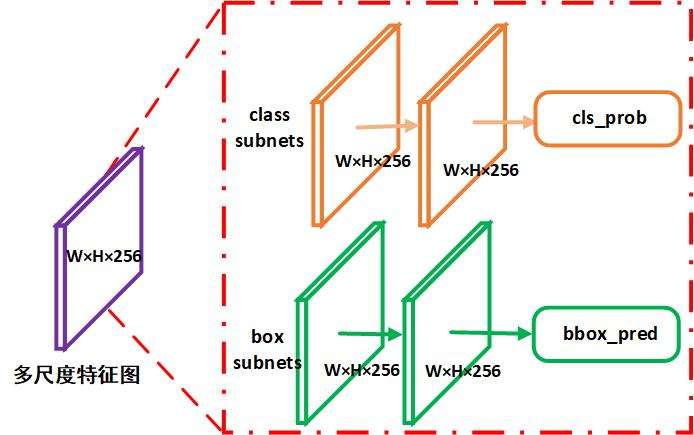
\includegraphics[width=0.95\linewidth, height=0.85\linewidth]{cls_reg1.jpg}
    \caption{}
	\end{subfigure}
  \centering
	\begin{subfigure}{0.45\linewidth}
		\centering
		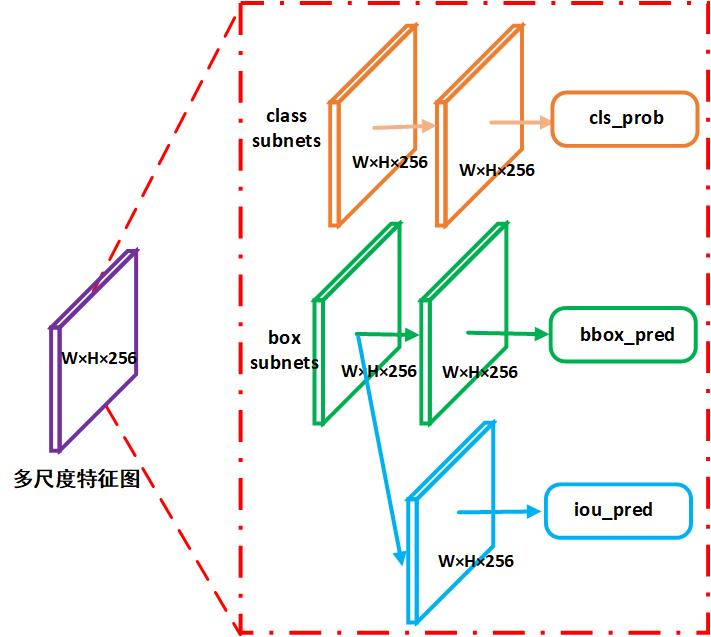
\includegraphics[width=0.95\linewidth, height=0.85\linewidth]{cls_reg2.jpg}
    \caption{}
	\end{subfigure}
  \caption{交并比预测分支结构}
	\label{fig:cls_reg}
\end{figure}

在训练过程,我们优化的目标有分类,坐标回归与交并比,损失函数如式~\ref{eq:loss_all}所示,其中${{L_{IoU}}(io{u_i},io{u_i}^*)}$定义为预测IoU和真实IoU之间的二元交叉熵损失。
\begin{equation}   
  Loss = \sum\limits_i {{L_{cls}}} \left( {{p_i},p_i^*} \right) + {\lambda _1}\sum\limits_i {p_i^*} {L_{reg}}\left( {{t_i},t_i^*} \right) + {\lambda _2}\sum\limits_i {{L_{IoU}}(io{u_i},io{u_i}^*)} 
  \label{eq:loss_all} 
\end{equation}

\subsection{训练标签分配策略}
  在目标检测网络训练过程中,标签分配(Label Assignment)是非常重要的一个流程。其目的是将训练样本划分为正负样本,并分配分类与回归的目标,
  计算其与真值之间的损失来监督训练。标签分配方式为网络训练提供了判别性的监督信号,决定了网络学习与收敛的方向,直接影响模型性能的好坏。
  本节介绍了我们训练过程中采用的不同标签分配策略,根据样本标签分配的正负权重设计,可以将这些方法划分为硬标签分配方法与软标签分配方法。

\subsubsection{硬标签分配策略}
硬标签分配策略假设每个锚框非正即负,若$w_{pos}, w_{neg}$分别表示样本属于正负样本的权重,则硬标签划分可以表示为
$w_{\text {pos }}, w_{n e g} \in\{0,1\}$且$w_{\text {pos }} +  w_{n e g} = 1$。这类方法的核心思想是找到一个最优划分
边界,将锚框分割为正样本集合与负样本集合。边界划分规则可以分为静态规则与动态规则这两类。

\subsubsection{最大交并比}
RetinaNet与Faster-RCNN等网络采用的是最常用的基于交并比最大化的标签分配策略(MaxIouAssigner)。
该方法有以下的几个步骤:(1)初始化,将正样本集合$P$、负样本集合$N$设置为空集,将所有锚框设置为忽略样本;
(2)计算多尺度特征图上所有锚框与所有真实框之间的交并比;(3)获取每个锚框交并比最大的GT框,如果交并比大于正样本阈值
(pos\_thres),则设置为正样本。如果小于负样本阈值(neg\_thres),则设置为负样本。(4)如果GT框没有被锚框匹配到,
则获得与GT框IOU最大的锚框,如果大于最小的正样本阈值,则将该锚框设置为正样本。

最大交并比标签分配策略是静态预先定义的标签分配方式。骨髓血细胞形状多变,比如杆状核粒细胞,通常呈现出U型,这导致目标的中心点
通常为背景,并不能代表这个目标,而按照最大交并比的方式会被判定为正样本,导致网络的性能较差。
\subsubsection{自适应样本选择}
自适应样本选择(Adaptive Training Sample Selection,ATSS)方法\cite{zhang2020bridging}基于L2距离与交并比动态计算分割阈值,是一种自适应划分
目标正负样本的标签分配策略。具体步骤如下:(1)对于网络输出的多个不同尺度特征图,在每个特征图上计算锚框中心坐标与目标中心
坐标的$L_2$距离,选取$K$个$L_2$距离最小的锚框作为候选的正样本,如果有$L$个层级的特征图,那么可以得到$K \times L$个候选正样本
。(2)计算每个候选正样本与目标真实框的交并比,得到一组交并比的数据。计算这组交并比的均值$m_g$与标准差$v_g$,将均值与标准差
相加,得到交并比的分割阈值$t_g = m_g + v_g$。(3)在每个层级的特征图的候选正样本中根据阈值,选择真正的正样本加入正样本集合中进行训练。

\begin{figure}[htbp]
	\centering
  \begin{subfigure}{0.48\linewidth}
    \centering
    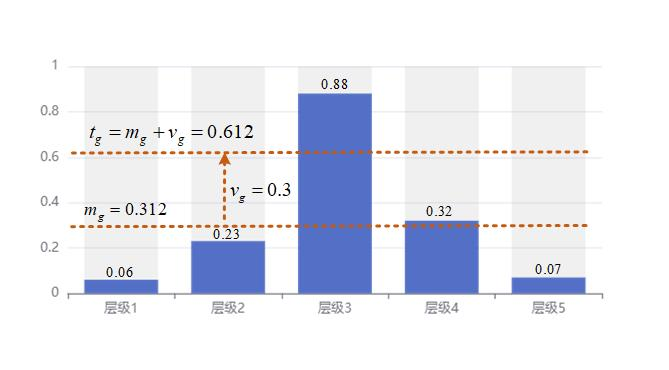
\includegraphics[width=1.0\linewidth, height=0.56\linewidth]{atss1.jpg}
    \caption{}
  \end{subfigure}
  \begin{subfigure}{0.48\linewidth}
    \centering
    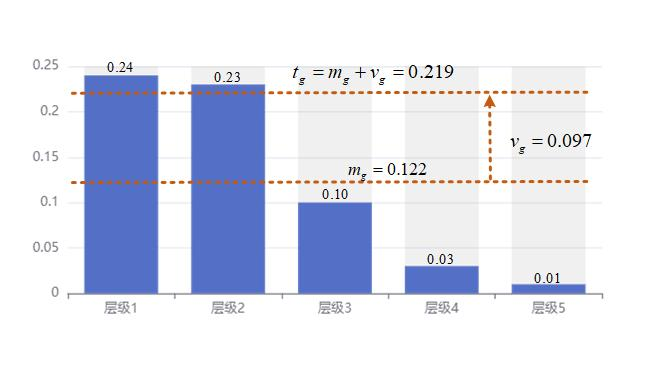
\includegraphics[width=1.0\linewidth, height=0.56\linewidth]{atss2.jpg}
    \caption{}
  \end{subfigure}
\caption{自适应样本选择阈值计算示意图}
	\label{fig:atss}
\end{figure}

图~\ref{fig:atss}为ATSS自适应计算阈值的示意图,柱状图的横坐标表示不同层级特征图,纵轴为交并比。柱子上的数字表示这个层级特征图上
目标与最近$K$个锚框交并比的均值。均值$m_g$代表锚框与目标真实框的匹配程度,如果$m_g$比较大,则候选正样本的质量都很好,
可以适当提高阈值来挑选更好正样本。均值低则应当降低分割阈值。标准差$v_g$表示特征层次锚框与目标真实框的匹配程度。如果标准差比较高,
则高质量的锚框集中在某一个层级的特征图中,应该提高阈值从最匹配的层级去挑选正样本。标准差比较低,说明所有层级的锚框匹配度都比较高,
可以设置一个比较低的阈值广泛的从多个层级的特征图中选取。

\subsubsection{概率标签分配}
概率标签分配(Probabilistic Anchor Assignment,PAA)\cite{kim2020probabilistic}锚框的得分数视为概率分布,并通过最大似然来估计分布参数,然后自适应的计算分割
阈值,来选取正负样本。锚框的分数用来衡量其与真实框的相似性,包括了分类得分与定位得分。分类得分是分类分支输出的置信度${P_i}(cls|\theta )$,定位得分为
预测框与真实框之间的交并比${\rm{IOU}}(f(a|\theta ),g)$,为平衡这两种得分的权重,引入$\lambda$参数。锚框得分如式~\ref{eq:score}所示:
\begin{equation}   
  S = {P_i}(cls|\theta ) \times {\rm{IOU}}{(f(a|\theta ),g)^\lambda } 
  \label{eq:score} 
\end{equation}

锚框可以分为正样本、负样本两组,因此可以使用双峰混合高斯分布来建模锚框的分数分布,如式~\ref{eq:gmm}所示。
\begin{equation}   
  P(a|g,\theta ) = {\phi _1}{\cal N}(a;{\mu _1},{\sigma _1}) + {\phi _2}{\cal N}(a;{\mu _2},{\sigma _2})
  \label{eq:gmm} 
\end{equation}

然后根据最大期望算法(Expectation-Maximization,EM)使得似然最大化。首先对参数$\phi_i, \mu_i, \sigma_i$进行随机初始化,
在E步中计算Q函数如式~\ref{eq:e_step}所示,式中$x_{1}, x_{2}, \ldots, x_{n}$为锚框的得分。
\begin{equation}   
  Q_{i}\left(z^{(i)}=k\right)=\frac{\phi_{k} \cdot \frac{1}{\sqrt{2 \pi} \sigma_{k}} \exp \left[-\frac{\left(x^{(i)}-\mu_{k}\right)^{2}}{2 \sigma_{k}^{2}}\right]}{\sum_{k=1}^{K} \phi_{k} \cdot \frac{1}{\sqrt{2 \pi} \sigma_{k}} \exp \left[-\frac{\left(x^{(i)}-\mu_{k}\right)^{2}}{2 \sigma_{k}^{2}}\right]}
  \label{eq:e_step} 
\end{equation}

在M步中根据式~\ref{eq:m_step}计算混合高斯分布的参数$\phi_1,\phi_2,\mu_1,\sigma_1,\mu_2,\sigma_2$。

概率标签分配的具体步骤如下:对于每个真实框,根据网络输出的置信度与坐标计算每个锚框的得分,在每个尺度的特征度选择K个得分最高的锚框。
采用最大期望算法去估计这组锚框的双峰高斯分布参数,找到两个最高峰对应横坐标的分数$s_1,s_2$,其中$s_1 < s_2$。将得分低于$s_1$的锚框
作为负样本。得分位于$s_1$与$s_2$之间的锚框划分为忽略样本,得分大于$s_2$的锚框作为正样本。最后那些没有参与分配的锚框均视为负样本。

\begin{equation}   
  \begin{aligned} \mu_{k} & =\frac{\sum_{i=1}^{N} Q_{k}^{(i)} x^{(i)}}{N_{k}} \\ 
    \sigma_{k} & =\frac{\sum_{i=1}^{N} Q_{k}^{(i)}\left(x^{(i)}-\mu_{(k)}\right)\left(x^{(i)}-\mu_{k}\right)^{T}}{N_{k}} \\ 
    \phi_{k} & =\frac{\sum_{i=1}^{N} Q_{k}^{(i)}}{N} \\ 
    N_{k} & =\sum Q_{k}^{N} Q_{k}^{(i)} 
  \end{aligned}
  \label{eq:m_step} 
\end{equation}
\subsubsection{最优输运标签分配}
最优输运\cite{villani2009optimal}标签分配将目标检测中的标签分配问题建模为
将标签从真实框输运到锚框代价最小的最优输运策略(Optimal Transport)问题,如图~\ref{fig:ota}所示。

最优输运问题的定义如下:假设有m个供应商与n个需求方,其中第$i$
个供应商有$a_i$单元的货物,第$j$个需求方需要$b_j$个单元的货物。每个单元的货物从第$i$个供应商运输到第$j$个的需求方的输运代价是$C_{ij}$。
最优输运的目标是找到一种输运计划$\mathbf{P}^{*}=\left\{P_{i, j} \mid i=1,2, \ldots m, j=1,2, \ldots n\right\}$将供应商的货物全部运输到需求方,
并使得运输的代价最小,其中$P_{i, j}$表示第$i$个供应商运输到第$j$个的需求方单元货物的数量。

\begin{figure}[htbp]                     
  \centering                      
  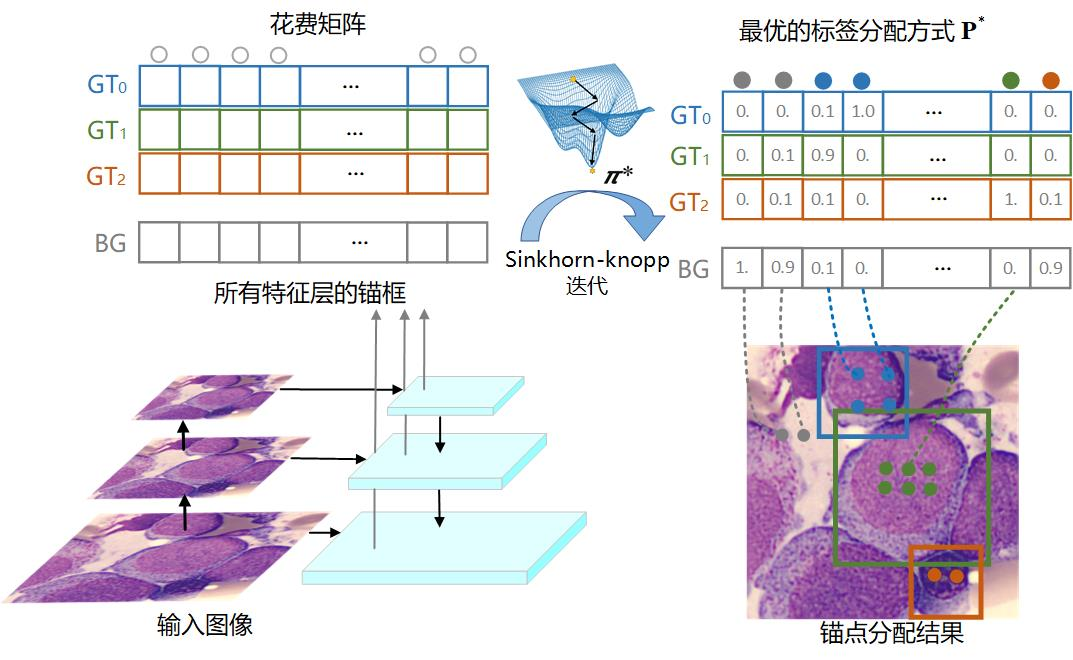
\includegraphics[width=0.95\linewidth]{ota.jpg}                      
  \caption{基于最优输运的标签分配策略}                      
  \label{fig:ota}       
\end{figure}  

最优输运的优化目标如式~\ref{eq:ota}所示:
\begin{equation}   
  \min _{\mathbf{P}} \sum_{i=1}^{m} \sum_{j=1}^{n} C_{i j} P_{i j} \quad P_{i j} \geq 0,i=1,2, \ldots m, j=1,2, \ldots n .
  \label{eq:ota} 
\end{equation}

其中第i的供应商输出的数量等于$s_i$,即$ \sum_{j=1}^{n} P_{i j}=a_{i}$。第j个需求方接收的数量等于$b_j$,即$\sum_{i=1}^{m} P_{i j}=b_{j}$。
供应商供应的数量等于需求方接收的数量$\sum_{i=1}^{m} a_{i}=\sum_{j=1}^{n} b_{j}$。

最优输运问题可以在多项式的时间复杂度内,通过Sinkhorn快速迭代的方法进行求解。该方法的思想源于交叉熵与对偶问题,定义$\mathbf{H}(\mathbf{P}) \stackrel{\text { def. }}{=} -\sum_{i, j} \mathbf{P}_{i, j}\left(\log \left(\mathbf{P}_{i, j}\right)-1\right)$
上述问题添加了拉格朗日算子和扰动项的形式如式~\ref{eq:ota_1}所示:
\begin{equation}   
  {\cal E}({\bf{P}},{\bf{f}},{\bf{g}}) = \sum\limits_{i = 1}^m {\sum\limits_{j = 1}^n {{{C}_{ij}}} } {{P}_{ij}} - \varepsilon {\bf{H}}({\bf{P}}) + {f_j}\left( {\sum\limits_{i = 1}^m {P_{ij}}  - {b_j}} \right) + {g_i}\left( {\sum\limits_{j = 1}^n {P_{ij}}  - {a_i}} \right)
  \label{eq:ota_1} 
\end{equation}

其中$\varepsilon$是一个常量超参数,控制熵正则化项的强度,实验中设置为0.1,$f_{j}(j=1,2, \ldots n)$与$g_{i}(i=1,2, \ldots, m)$是拉格朗日乘子。
通过使得目标函数导数等于零求得最优的输运策略如式~\ref{eq:ota_2}所示:
\begin{equation}   
  \frac{\partial \mathcal{E}(\mathbf{P}, \mathbf{f}, \mathbf{g})}{\partial P_{i, j}}=C_{i, j}+\varepsilon \log \left(P_{i, j}\right)-f_{j}-g_{i}=0
  \label{eq:ota_2} 
\end{equation}

因此最优输运策略为$\mathbf{P}^{*}$如式~\ref{eq:ota_3}所示:
\begin{equation}   
  P_{ij}^* = \exp \left( { - \frac{{{f_j}}}{\varepsilon }} \right)\exp \left( { - \frac{{{C_{ij}}}}{\varepsilon }} \right) \exp \left( { - \frac{{{g_i}}}{\varepsilon }} \right)
  \label{eq:ota_3} 
\end{equation}

令$s_j=\exp \left( { - \frac{{{f_j}}}{\varepsilon }} \right)$, $U_{ij}=\exp \left( { - \frac{{{C_{ij}}}}{\varepsilon }} \right)$,$t_i=\exp \left( { - \frac{{{g_i}}}{\varepsilon }} \right)$
上述变量满足如式~\ref{eq:ota_4}的约束关系:
\begin{equation}   
  \begin{array}{l}
  \sum_{i} P_{i j}=s_{j}\left(\sum_{i} U_{i j} t_{i}\right)=b_{j} \\
  \sum_{j} P_{i j}=\left(s_{j} \sum_{i} U_{i j}\right) t_{i}=a_{i}
  \end{array}
  \label{eq:ota_4} 
\end{equation}

上式的约束关系需要同时满足,因此$t_i$与$s_j$的交替迭代公式如下:
\begin{equation}   
  s_j^{l + 1} = \frac{{{b_j}}}{{\sum\limits_i {{U_{ij}}} t_i^l}},\quad t_i^{l + 1} = \frac{{{a_i}}}{{\sum\limits_j {{U_{ij}}} s_j^{l + 1}}}
  \label{eq:ota_5} 
\end{equation}

在目标检测的背景下,假设一张图片中有$m$个真实框,检测网络所有的FPN层总共输出了$n$个锚框。将真实框
视为供应商,可以为$k$个锚框提供正样本的标签,等价于有$k$个单元的货物$\text { i.e., } a_{i}=k, i=1,2, \ldots, m$。
每个锚框视为需求方,需要一个标签$\text { i.e., } b_{j}=1, j=1,2, \ldots, n$。此外引入一个背景供应商,来为锚框提供
负样本标签,数量为$n - m \times k$。

将正样本标签从某一个真实框$gt_{i}$输运到一个锚框$anchor_j$的代价定义为分类与回归的加权损失,如式~\ref{eq:ota_cost_fg}所示:
\begin{equation}   
  C_{ij}^{fg} = {L_{cls}}\left( {p_i^*,p_j^{cls}(\theta )} \right) + \lambda {L_{reg}}\left( {t_i^*,t_j^{box}(\theta )} \right)
  \label{eq:ota_cost_fg} 
\end{equation}

其中$\theta$代表模型参数,$p_j^{cls}(\theta )$与$t_j^{box}(\theta )$分别代表模型预测的分类得分与坐标回归值。
$p_i^*$与$t_i^*$代表了真实类别与坐标。$L_{cls}$与$L_{reg}$为交叉熵损失函数与GIOU损失函数。

背景供应商将一个负样本标签传递到锚框的花费为分类损失,如下式所示:
\begin{equation}   
  C_j^{bg} = {L_{cls}}\left( {\Phi ,p_j^{cls}(\theta )} \right)
  \label{eq:ota_cost_bg} 
\end{equation}

在定义好花费矩阵后,最优输运的策略$\mathbf{P^*}$可以可以通过Sinkhorn-Knopp迭代算法进行求解。每个anchor的标签
为最大的标签所对应的供应商类别。算法流程如算法~\ref{alg:alg_ota}所示。

\renewcommand{\algorithmicrequire}{\textbf{输入:}\unskip}
\renewcommand{\algorithmicensure}{\textbf{输出:}\unskip}
\begin{algorithm}[htbp]
  \caption{最优输运标签分配} % 名称
  \label{alg:alg_ota}
  \begin{algorithmic}[1]
    \REQUIRE
      ~\\
      $I$: 输入图像            \\
      $A$: 网络输出的一组锚框   \\
      $G$: 图像中目标真实框标注 \\
      $\varepsilon$: Sinkhorn-Knopp迭代熵正则化项 \\
      $T$: Sinkhorn-Knopp迭代次数 \\
      $\lambda$: 式~\ref{eq:ota_cost_fg}中的平衡因子 
    \ENSURE
      ~\\
      $\mathbf{P^*}$标签最优输运策略
      \STATE set $m = |G|$, $n = |A|$;
      \STATE 网络前向计算每个锚框的分数与坐标$P^{cls}, P^{box}$
      \STATE 动态计算每个GT框的$a_i$
      \STATE 计算得到背景供应商的标签数量$a_{m + 1} = n-\sum_{i=1}^{m} a_{i}$
      \STATE $b_j(j = 1, 2 \dots n)$使用1初始化
      \STATE 前景分类损失$C_{ij}^{cls} = FocalLoss(P_{j}^{cls}, G_{i}^{cls})$
      \STATE 前景回归损失$C_{ij}^{reg} = IoULoss{P_{j}^{box}, G_{i}^{box}}$
      \STATE 背景花费$C_{bg}^{cls} = FocalLoss(P_{j}^{cls}, \Phi)$
      \STATE 前景花费$C_{fg} = C^{cls} + \lambda C^{reg}$
      \STATE 计算最终的花费矩阵将$C_{bg}$拼接到$C_{fg}$的最后一行
      \STATE 对$s^0, t^0$进行随机初始化
      \FOR {$i = 1$; $i < T$; $i++$ }
        \STATE 计算$s^{l+1}, t^{l+1} \leftarrow \operatorname{SinkhornIter}\left(C, s^{l}, t^{l}, a, b\right)$
     \ENDFOR
      \STATE 根据式~\ref{eq:ota_3}, 计算并返回最优的标签分配策略$\mathbf{P}^*$
  \end{algorithmic}
\end{algorithm}
% \subsubsection{软标签分配策略}
% \subsection{完全动态标签分配}
% \subsection{损失函数}

\section{算法实现与实验结果分析}
\subsection{实验环境}
训练平台使用linux,操作系统为ubuntu20.04,GPU为NVIDIA$\enspace$RTX3090,CPU为Intel(R)$\enspace$Core(TM)$\enspace$i9-10940X。深度学习框架为Pytorch1.13.1,
训练的批量大小设置为16。使用SGD随机梯度下降优化器对网络参数进行更新,动量设置为0.9,权重衰减设置为5e-4。初始化的学习率为0.001。
网络总共训练36个轮次,在第16与第28个轮次,学习率变为原来的$1/10$。RetianNet中Focal Loss中正负样本平衡参数$\alpha=0.25$,难易调整参数$\gamma=2$。
主干网络使用在coco数据集上预训练的ResNet50网络。

\subsubsection{数据集介绍}
骨髓血细胞图像来自邃蓝智能科技(上海)有限公司合作医院提供,首先采用第2.1小节阐述的主动学习标注策略进行边界框的标注。
我们总共标记了6821张血细胞图像,训练集与测试集按照4:1的比例进行随机划分,训练集包含了5456张图像,测试集包含了1365张图像。
通常每个图像中包含1到10个有核血细胞,数据集总共标记了11352个血细胞,训练集有9065个血细胞,测试集有2287个血细胞。数据集的分布如
表~\ref{table:cell_detect1}所示:

\begin{table}[htbp]
  \caption{骨髓血细胞检测数据集分布}   
  \centering 
  \label{table:cell_detect1}
  \begin{tabular}{ccccc}
    \toprule[1pt]
    序号 & 类别名  &  类别简写 & 训练集数量 & 测试集数量 \\
    \midrule[1pt] 
    1 & 原始细胞 & Prim & 1856 & 467 \\ 
    2 & 淋巴细胞 & Lym & 996 & 226   \\ 
    3 & 单核细胞 & Mono & 206 & 52   \\ 
    4 & 浆细胞 & Plas & 272 & 70   \\ 
    5 & 红细胞 & Red & 1880 & 503   \\ 
    6 & 早幼粒细胞 & Promy & 357 & 107   \\ 
    7 & 嗜中性中幼粒细胞 & Myelo & 701 & 150   \\ 
    8 & 嗜中性晚幼粒细胞 & Late & 503 & 144   \\ 
    9 & 嗜中性杆状核细胞 & Rods & 998 & 241   \\  
    10 & 嗜中分叶核细胞 & Lobu & 821 & 195   \\  
    11 & 嗜酸性粒细胞 & Eosl & 475 & 132   \\  
    \hline
    总计 &   &   & 9065 & 2287 \\
    \bottomrule[1pt]      
  \end{tabular} 
\end{table}

\subsection{实验结果与分析}
\subsubsection{评价指标} 
在\ref{section:detect}节中,我们提出了先检测、再识别的骨髓血细胞计算处理流程。在本节中,我们只关注血细胞检测的准确性,网络性能评估指标采用准确率、召回率、
平均精度均值(mAP)与PR曲线,具体定义见~\ref{section:metrics}节。
\subsubsection{实验结果}
为了验证本节提出的改进RetinaNet方法在骨髓血细胞检测上的有效性,我们在上节所提的骨髓血细胞数据集上进行测试,在不同交并比阈值条件下,
网络的准确率、召回率、f1-score、平均检测精度均值与FPS如表~\ref{table:cell_det}所示,其中准确率、召回率为f1-score最大条件下对应的数值,FPS是网络每秒可计算的图像帧数量。

从表中我们可以看到,本节提出的改进模型效果较好,在交并比为0.75的条件下,f1-score为0.9474,召回率为0.950,准确率为0.9448。
随着交并比的逐渐增大,网络的准确率与召回率均开始下降,在交并比为0.95时,下降最为明显,平均检测精度只有0.176。因此,对于高精度的定位(IOU>0.9),模型检测性能仍有待提升,我们认为
未来可以在数据量上进行扩充,此外在标注上进行更加精细化的校对。
\begin{table}[htb]
  \caption{改进RetinaNet骨髓血细胞检测结果}   
  \centering 
  \label{table:cell_det}
  \begin{tabular*}{0.90\hsize}{@{}@{\extracolsep{\fill}}cccccc@{}}
    \toprule[1pt]
    IOU & 准确率  &  召回率& f1-score & mAP & FPS \\
    \midrule[1pt] 
    0.5  & 0.9624 & 0.96 & 0.9612 & 0.9864 & 27.2 \\
    0.55 & 0.9594 & 0.96 & 0.9597 & 0.9837 & 27.2 \\
    0.6  & 0.9594 & 0.96 & 0.9597 & 0.9837 & 27.2 \\
    0.65 & 0.9579 & 0.96 & 0.9589 & 0.9821 & 27.2 \\
    0.7  & 0.9559 & 0.95 & 0.9529 & 0.9735 & 27.2 \\
    0.75 & 0.9448 & 0.95 & 0.9474 & 0.9668 & 27.2 \\
    0.8  & 0.931  & 0.92 & 0.9255 & 0.9328 & 27.2 \\
    0.85 & 0.8738 & 0.86 & 0.8668 & 0.8463 & 27.2 \\
    0.9  & 0.7256 & 0.72 & 0.7228 & 0.6305 & 27.2 \\
    0.95 & 0.3537 & 0.33 & 0.3414 & 0.1766 & 27.2 \\
    \bottomrule[1pt]      
  \end{tabular*} 
\end{table}

此外,我们对比了SSD512\cite{liu2016ssd}、Faster-RCNN\cite{ren2015faster}、Cascade-RCNN\cite{cai2018cascade}、
RetinaNet\cite{lin2017focal}、YOLOV3\cite{redmon2018yolov3}与DETR\cite{zhu2020deformable}等六种基于深度学习的主流目标检测网络,
这些网络均使用在COCO数据集上预训练模型进行参数初始化,然后基于迁移学习在骨髓血细胞检测数据集上进行微调。表~\ref{table:cell_det_con}为不同网络的平均检测精度对比,
其中$AP_{50}$表示在交并比为0.5条件下的平均检测精度。

从表~\ref{table:cell_det_con}中我们可以看到,SSD512网络检测精度最差,这是由于VGG16骨干网络特征表达能力相比与ResNet等
残差网络更差。在交并比为0.5的条件下,DETR网络的平均精度最高,本节提出的网络略低于DETR方法。
在交并比为0.75与0.9的条件下,本节的方法均高于其他对比方法,特别是在交并比为0.9的条件下,本节方法 
相比与次优的Cascade-RCNN方法提升了约6.93\%。该结果说明Cascade-RCNN通过级联RPN网络的方式,可以有效的
提升候选框的定位质量,而本文提出的改进点将IOU交并比纳入到检测网络的推理阶段,也可以帮助网络找到定位精度更好
的候选框。在网络的计算量与参数量方面,DETR的计算量最低,SSD512的参数量最少,本文提出的改进方法相比与基础RetinaNet
方法计算量增加了3.8\%,参数量增加了1.58MB。总而言之,本节提出的改进RetinaNet方法在骨髓血细胞的检测精度上要优于其他方法,
交并比为0.75条件下的平均检测精度提升了1.26\%。

本节提出的改进模型在骨髓血细胞数据集上检测的可视化结果如图~\ref{fig:detect_res}所示,图中将置信度阈值大于0.5的骨髓血细胞以红色检测框标出,左上角的
数字为置信度分数,从图中我们可以看到,该网络可以有效的对密集与黏连的血细胞区域进行检测。
\begin{table}[htb]
  \caption{不同目标检测方法在骨髓血细胞测试集上的性能对比}   
  \centering 
  \label{table:cell_det_con}
  \begin{tabular*}{0.90\hsize}{@{}@{\extracolsep{\fill}}ccccccc@{}}
    \toprule[1pt]
    方法 & 主干网络  &  $AP_{50}$ & $AP_{75}$ & $AP_{90}$ & \makecell{参数量大小\\(MB)} & \makecell{运算次数 \\(GFLOPs)} \\
    \midrule[1pt] 
    SSD512      & VGG16    & 0.9748 & 0.9178 & 0.3234 &  36.04 & 250.92 \\
    Faster-RCNN & ResNet50 & 0.9819 & 0.9458 & 0.4965 &  41.17 & 139.25 \\ 
    Cascade-RCNN & ResNet50 & 0.9806& 0.9556 & 0.5896 & 69.17 & 167.24   \\ 
    RetinaNet   & ResNet50 & 0.9801 & 0.9542 & 0.5215 &  36.31 & 135.73  \\ 
    YOLOV3      & DarkNet53 & 0.9794 & 0.9508 & 0.4646 & 61.95 & 127.11  \\ 
    DETR        & ResNet50 & 0.9888 &  0.9559 & 0.5844 &  41.30 & 59.82  \\ 
    \hline
    本节提出的网络 & ResNet50 & 0.9864 & 0.9668 &  0.6305 & 37.89 & 140.94\\
    \bottomrule[1pt]      
  \end{tabular*} 
\end{table}
\begin{figure}[htb]
	\centering
  \begin{subfigure}{0.24\linewidth}
    \centering
    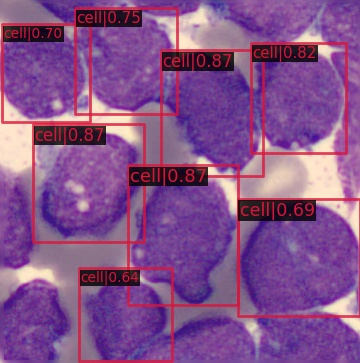
\includegraphics[width=0.95\linewidth, height=0.95\linewidth]{detect_result/1.jpg}
  \end{subfigure}
	\centering
  \begin{subfigure}{0.24\linewidth}
    \centering
    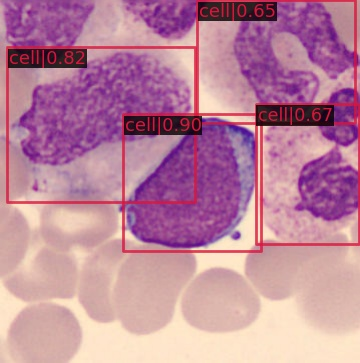
\includegraphics[width=0.95\linewidth, height=0.95\linewidth]{detect_result/2.jpg}
  \end{subfigure}
		\centering
  \begin{subfigure}{0.24\linewidth}
    \centering
    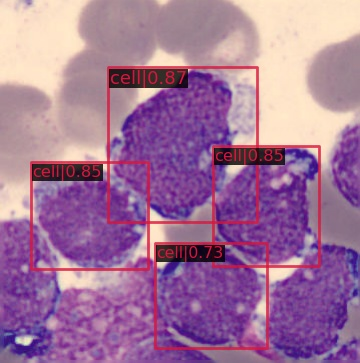
\includegraphics[width=0.95\linewidth, height=0.95\linewidth]{detect_result/3.jpg}
  \end{subfigure}
		\centering
  \begin{subfigure}{0.24\linewidth}
    \centering
    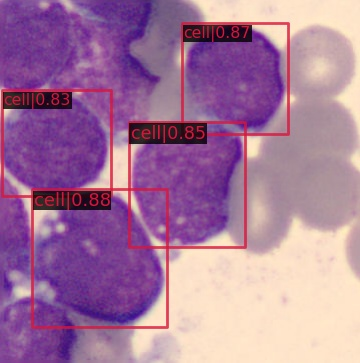
\includegraphics[width=0.95\linewidth, height=0.95\linewidth]{detect_result/4.jpg}
  \end{subfigure}
\\	
\vspace{0.2cm}
	\centering
  \begin{subfigure}{0.24\linewidth}
    \centering
    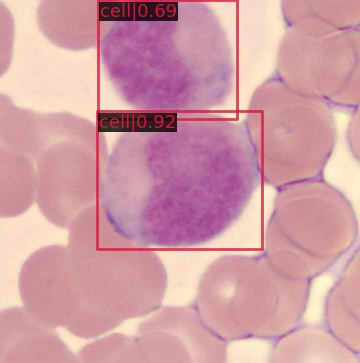
\includegraphics[width=0.95\linewidth, height=0.95\linewidth]{detect_result/5.jpg}
  \end{subfigure}
		\centering
  \begin{subfigure}{0.24\linewidth}
    \centering
    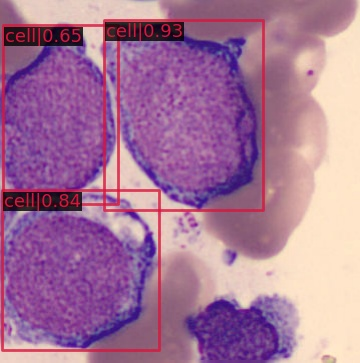
\includegraphics[width=0.95\linewidth, height=0.95\linewidth]{detect_result/6.jpg}
  \end{subfigure}
		\centering
  \begin{subfigure}{0.24\linewidth}
    \centering
    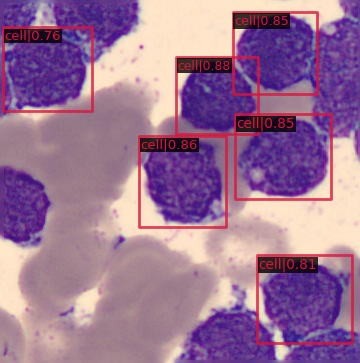
\includegraphics[width=0.95\linewidth, height=0.95\linewidth]{detect_result/7.jpg}
  \end{subfigure}
		\centering
  \begin{subfigure}{0.24\linewidth}
    \centering
    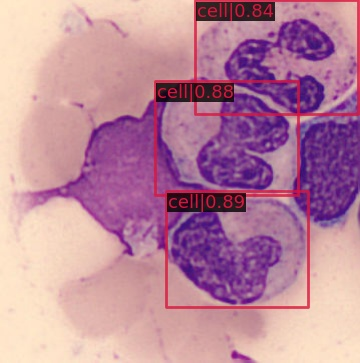
\includegraphics[width=0.95\linewidth, height=0.95\linewidth]{detect_result/8.jpg}
  \end{subfigure}
  \caption{骨髓血细胞数据集上的检测结果}
	\label{fig:detect_res}
\end{figure}

\subsubsection{改进网络结构}
为了验证本节提出了全局注意力路径聚合网络模块与IOU预测分支网络模块的有效性,我们分别在基线模型上添加单一模块来验证这两种模块的有效性。
不同模型在骨髓血细胞测试集的结果如表~\ref{table:net_ablation}所示,$AP_{50}$、$AP_{75}$与$AP_{90}$分别表示交并比为0.5、0.75与0.9条件下的平均检测精度。
√代表网络添加该模块, ×代表网络不包含该模块,上述模型均使用最大交并比(MaxIOU)的标签分配策略。
\begin{table}[htbp]
  \caption{骨髓血细胞检测网络模块消融实验}   
  \centering 
  \label{table:net_ablation}
  \begin{tabular*}{0.90\hsize}{@{}@{\extracolsep{\fill}}cccccc@{}}
    \toprule[1pt]
    主干网络  & 路径聚合模块 & IOU预测模块 &$AP_{50}$ & $AP_{75}$ & $AP_{90}$ \\
    \midrule[1pt] 
    RetinaNet    & × & × & 0.9801 & 0.9542 &  0.5215  \\
    RetinaNet    & √ & × & 0.9893 & 0.9601 &  0.5951  \\ 
    RetinaNet    & × & √ & 0.9843 & 0.9575 & 0.5831     \\ 
    RetinaNet    & √ & √ & 0.9856 & 0.9629 &  0.6137  \\ 
    \bottomrule[1pt]      
  \end{tabular*} 
\end{table}

从表~\ref{table:net_ablation}中,我们可以看到,单独添加路径聚合网络模块,网络在交并比为0.5条件下的平均检测精度最高,
在交并比为0.75与0.9时,平均检测精度相比于基线模型提升了0.59\%与7.36\%。单独添加IOU预测模块,在交并比为0.75与0.9时,
平均检测精度分别提升了0.33\%与6.16\%,实验结果表明在网络结构中引入路径聚合网络与IOU预测网络均可以有效提高骨髓血细胞
的检测精度。组合两种模块后的网络在交并比为0.75条件下的平均检测精度为0.9629,相比于基线模型提升了0.87 \%。
在交并比为0.90条件下的平均检测精度为0.6137,相比于基线模型提升了9.22\%。
\subsubsection{标签分配策略}
在本小节,我们对比了不同的标签分配策略对骨髓血细胞检测精度的影响,实验中网络结构使用改进的RetinaNet网络,
四种标签分配策略分别是最大交并比(MaxIOU)、自适应样本选择(ATSS)、概率标签分配(PAA)与最优输运标签分配(OTA)。
在骨髓血细胞检测数据集上的结果如表~\ref{table:assign_ablation}所示,表中$AP_{50}$、$AP_{75}$与$AP_{90}$的定义同表~\ref{table:net_ablation},
$AR_{50}$、$AR_{75}$与$AR_{90}$分别表示置信度阈值大于0.3、单张图像最大检测框数量为100、交并比为0.5、0.75、0.9条件下的
召回率。
\begin{table}[htbp]
  \caption{标签分配策略消融实验}   
  \centering 
  \label{table:assign_ablation}
  \begin{tabular*}{1.0\hsize}{@{}@{\extracolsep{\fill}}cccccccc@{}}
    \toprule[1pt]
    主干网络  & 标签分配策略 & $AP_{50}$ & $AP_{75}$ & $AP_{90}$ & $AR_{50}$ & $AR_{75}$ & $AR_{90}$ \\
    \midrule[1pt] 
    改进RetinaNet    & MaxIOU & 0.9856 & 0.9629 &  0.6137  & 1.00   & 0.9784 & 0.7170 \\
    改进RetinaNet    & ATSS   & 0.9845 & 0.9657 &  0.6235  & 1.00   & 0.9825 & 0.7377\\ 
    改进RetinaNet    & PAA    & 0.9843 & 0.9656 &  0.6246  & 1.00   & 0.9831 & 0.7361 \\ 
    改进RetinaNet    & OTA    & 0.9864 & 0.9668 &  0.6305  & 1.00   & 0.9841 & 0.7372 \\ 
    \bottomrule[1pt]      
  \end{tabular*} 
\end{table}

从表中可以看到,ATSS、PAA与OTA的标签分配策略要优于基线模型的MaxIOU标签分配策略。在交并比为0.50的条件下四种标签策略的方法召回率均为1.00,
平均检测精度OTA最高,MaxIOU次之。在交并比为0.75与0.9的条件下,OTA标签分配方法在召回率与平均检测精度优于其他三种标签分配方法,ATSS与PAA方法
性能非常接近,MaxIOU方法效果最差。在交并比为0.75时,OTA标签分配方法相比于基线方法平均分类精度提升了0.39\%,在交并比为0.9时,召回率提升了2.02\%。
上述实验结果表明,最优输运标签分配策略可以有效避免模糊样本的出现,提高网络的召回能力并进一步提升平均检测精度。

\section{小结}
针对密集、黏连骨髓血细胞区域存在漏检、误检等问题,本节提出了一种基于改进RetinaNet的骨髓血细胞检测网络。
我们在基线模型上总共实现了三个创新改进点,第一点是基于全局注意力的自下而上的路径聚合模块,
该模块通过特征直连缩短了底层到顶层特征之间的信息传递路径,使得浅层纹理等高分辨定位信息可以更有效的传递到顶层,
该模块使得网络的$AP_{75}$提升了0.59\%。第二点,网络引入了IOU预测分支,对每个锚框与可能对应真实框交并比进行预测,
在推理阶段将检测框的定位质量纳入到非极大值抑制的考量中,该模块使得网络的$AP_{75}$提升了0.33\%。
第三点,本节探究了不同标签分配策略对检测性能的影响,将最优输运标签策略用于密集区域血细胞的标签分配,避免了模糊分配样本的出现,
提高网络对血细胞的召回能力。在骨髓血细胞测试集上的实验结果表明,本文提出的改进方法相比于基线模型在平均检测精度上提升了1.26\%,达到了较为先进的性能。
改进网络单张图像的平均检测时间约为37ms,可以用于实时自动化骨髓血细胞检测。


